
\begin{frame}{Logistic Regression package}

\begin{columns}[T]
\begin{column}{0.5\textwidth}
TODO -- Formact code

\texttt{alpha = 1   # Lasso = 1 -- Ridge = 0 -- 0 < Elastic < 1}
\texttt{cv.model = cv.glmnet(x.train, y.train, family = 'binomial', alpha = alpha)}
\texttt{best.lambda <- cv.model\$lambda.min}
\end{column}
\begin{column}{0.5\textwidth}
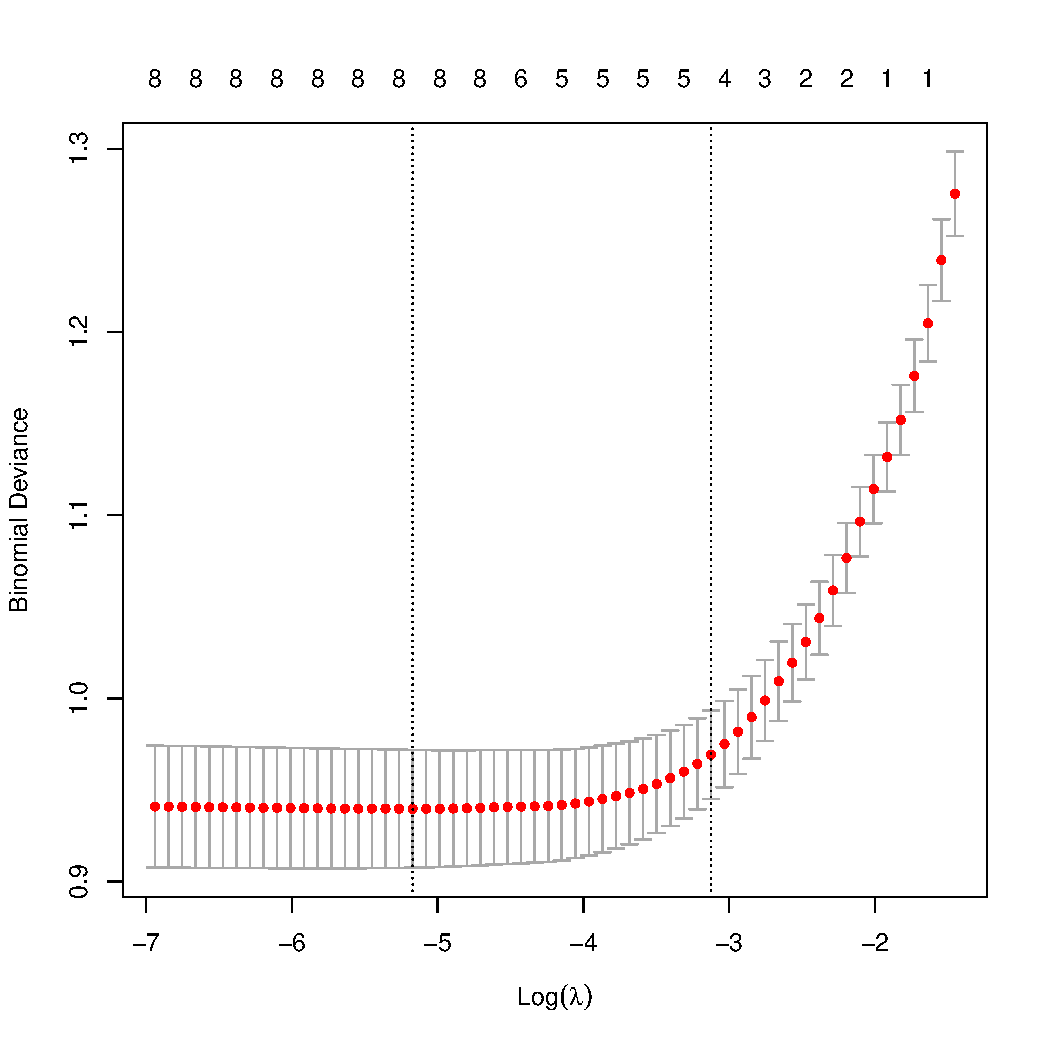
\includegraphics[width=0.85\columnwidth]{plots/cv_lambda.pdf}
\end{column}
\end{columns}

\end{frame}

\begin{frame}{Ridge and Lasso variable importance}

\vspace*{-1em}\begin{columns}[T]
\begin{column}{0.5\textwidth}
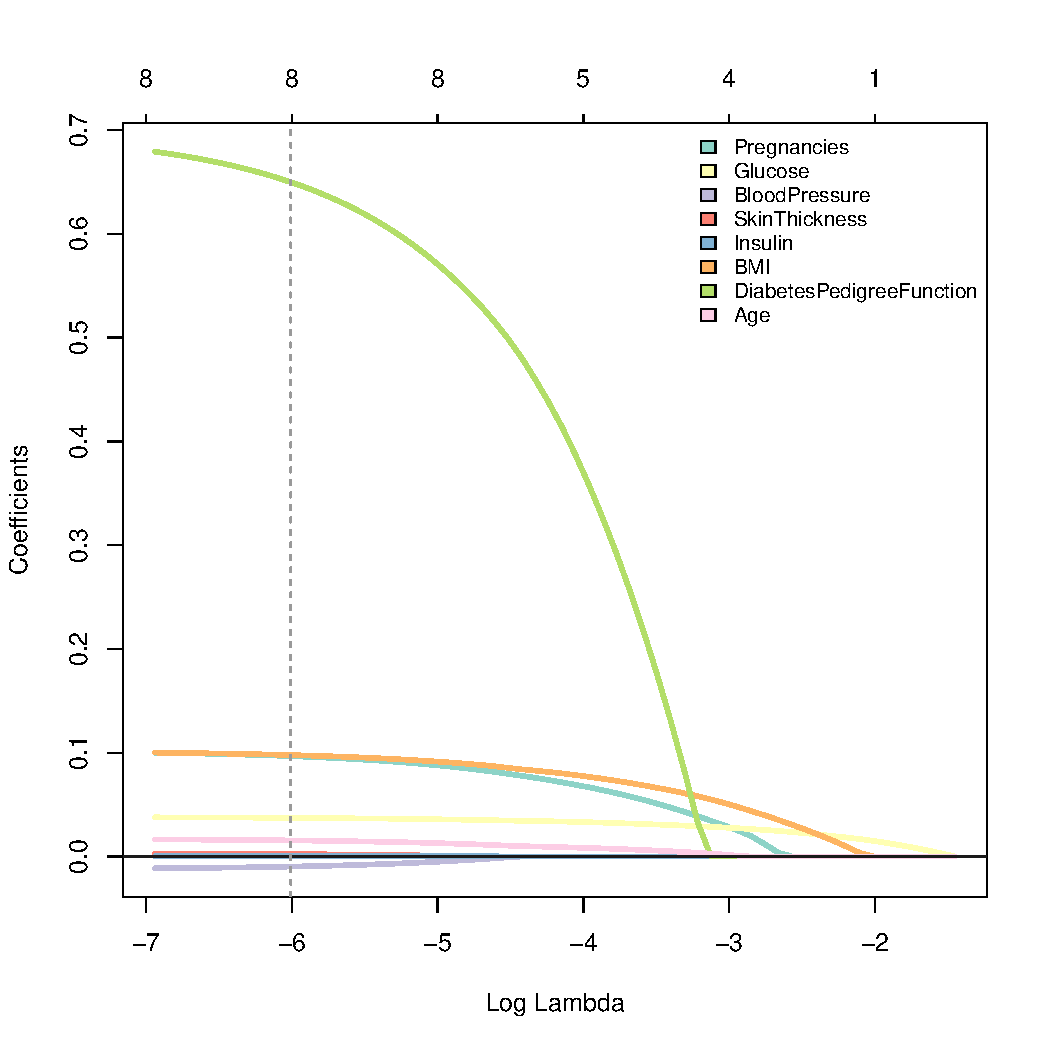
\includegraphics[width=0.85\columnwidth]{plots/diabetes_lasso.pdf}
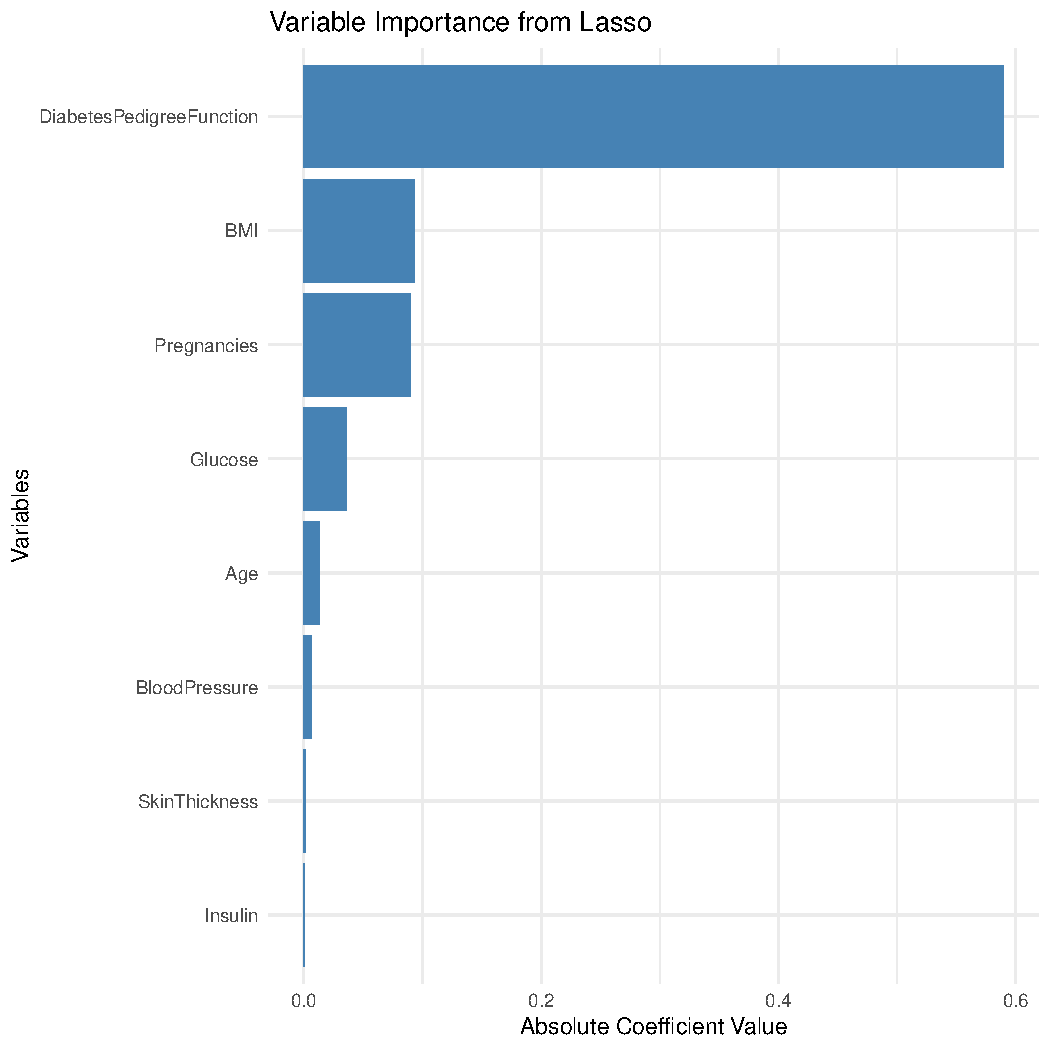
\includegraphics[width=0.7\columnwidth]{plots/variable_importance_lasso.pdf}
\end{column}
\begin{column}{0.5\textwidth}
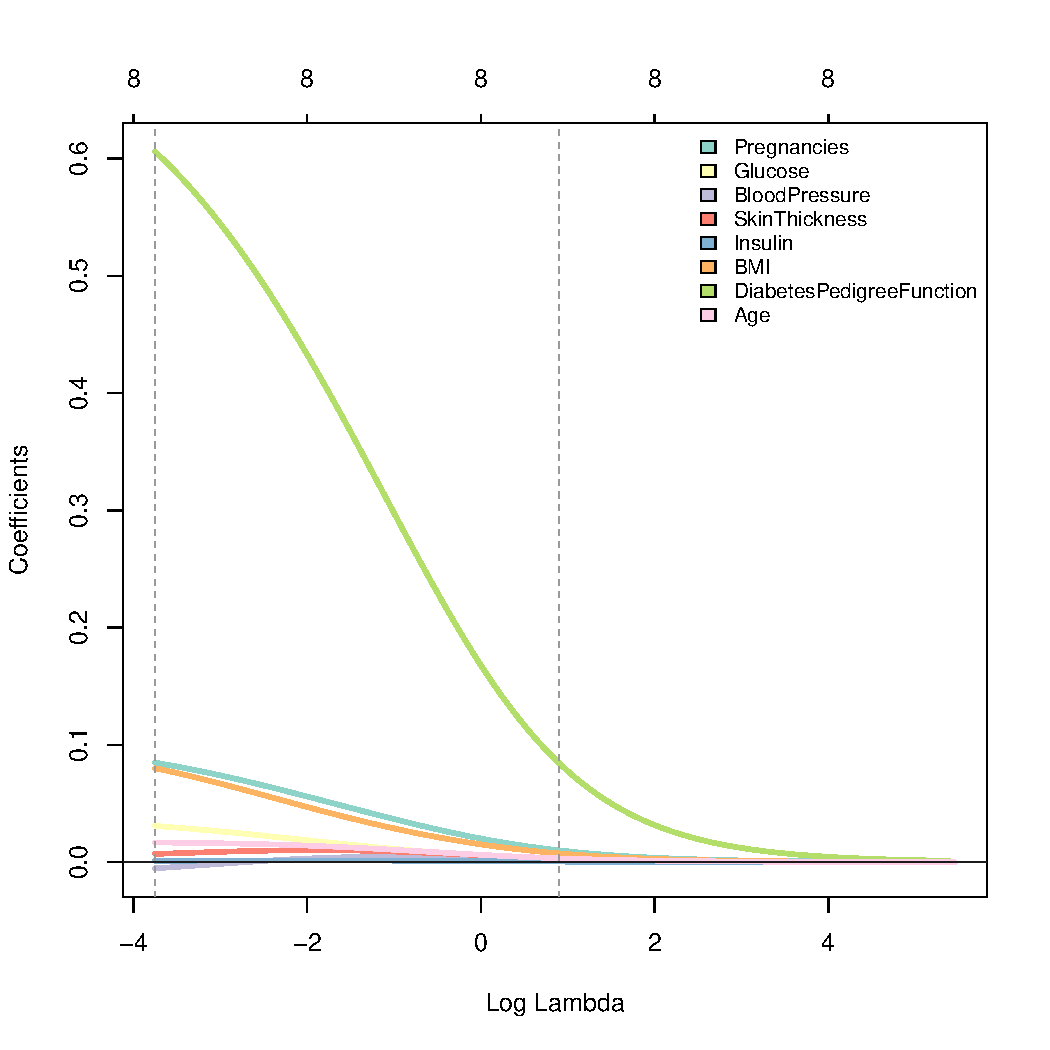
\includegraphics[width=0.85\columnwidth]{plots/diabetes_ridge.pdf}
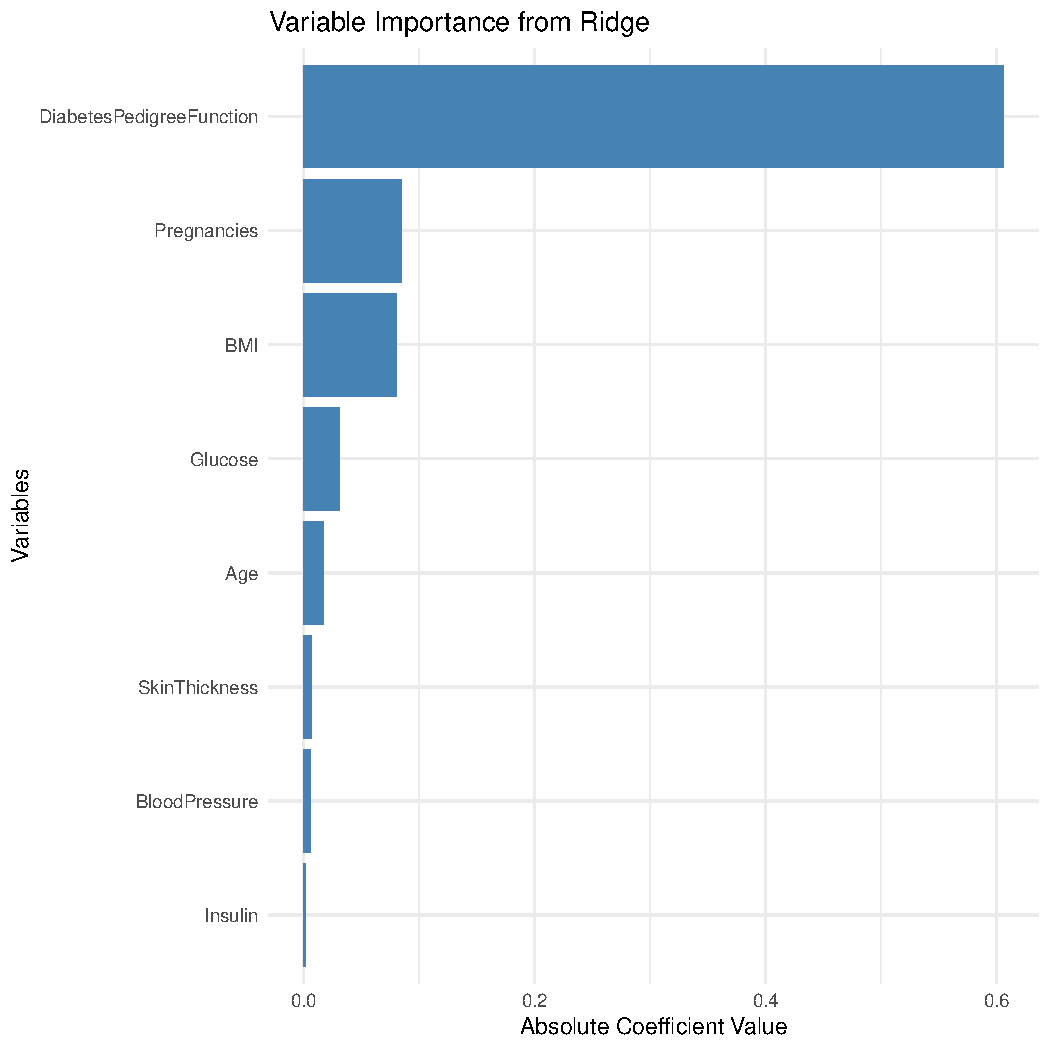
\includegraphics[width=0.7\columnwidth]{plots/variable_importance_ridge.pdf}
\end{column}
\end{columns}

\end{frame}

\begin{frame}{ElasticNet and AdaLasso variable importance}

\vspace*{-1em}\begin{columns}[T]
\begin{column}{0.5\textwidth}
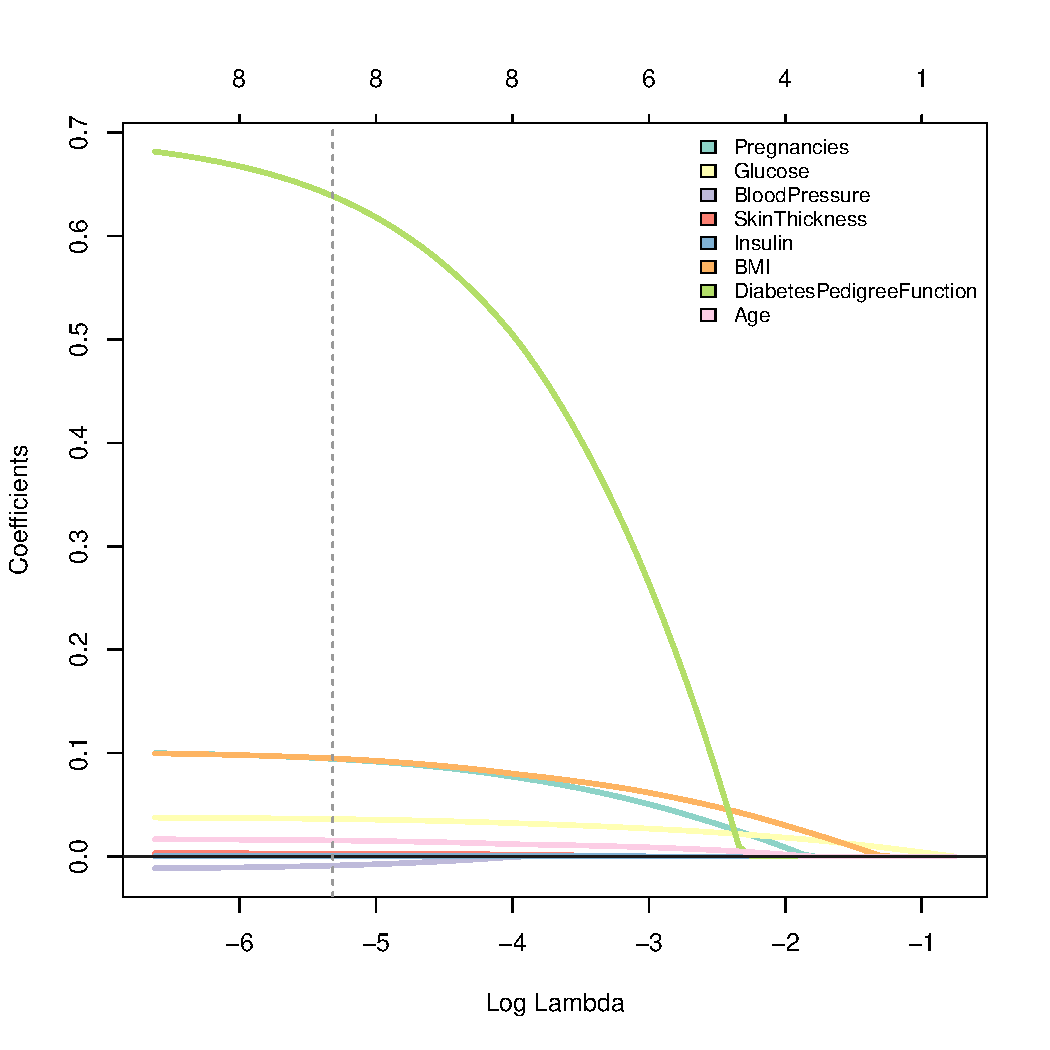
\includegraphics[width=0.85\columnwidth]{plots/diabetes_elasticnet.pdf}
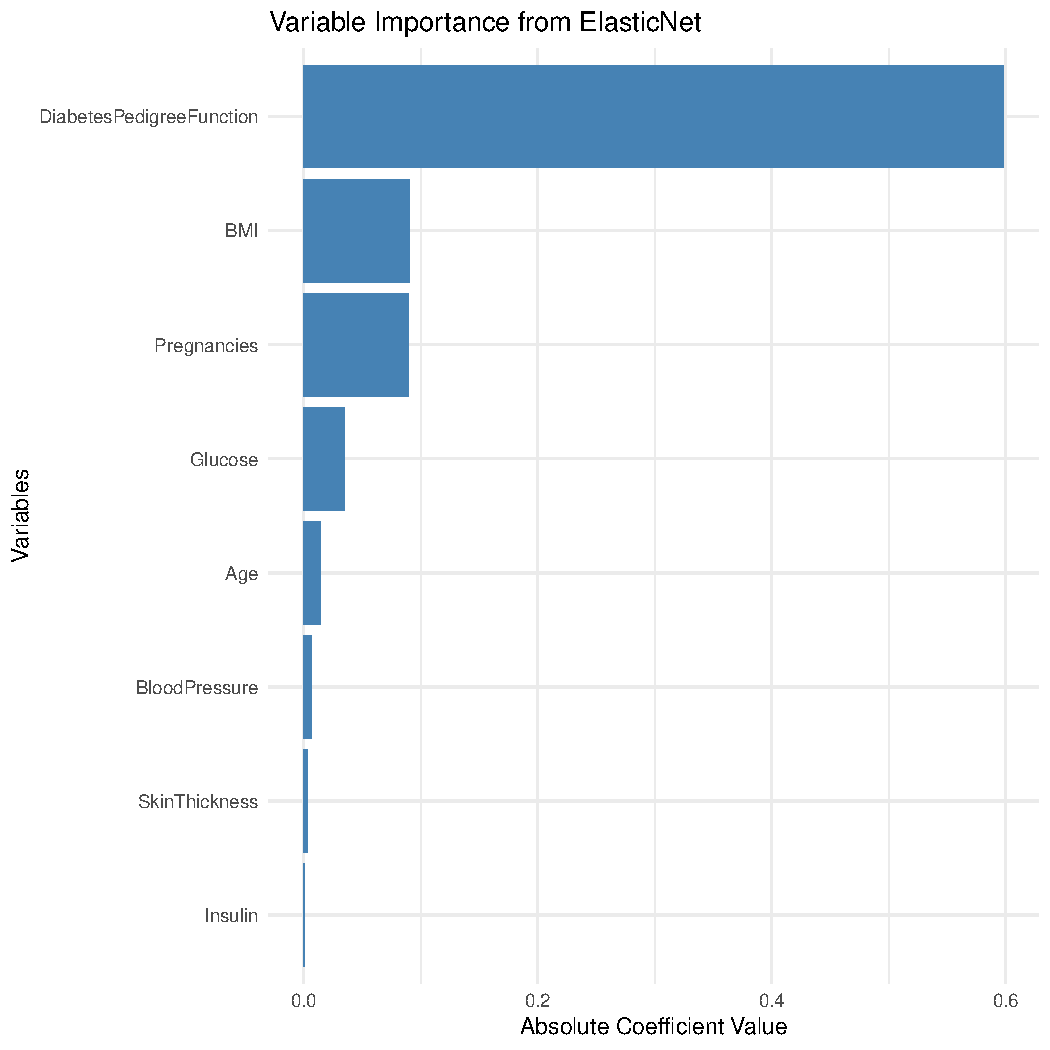
\includegraphics[width=0.7\columnwidth]{plots/variable_importance_elasticnet.pdf}
\end{column}
\begin{column}{0.5\textwidth}
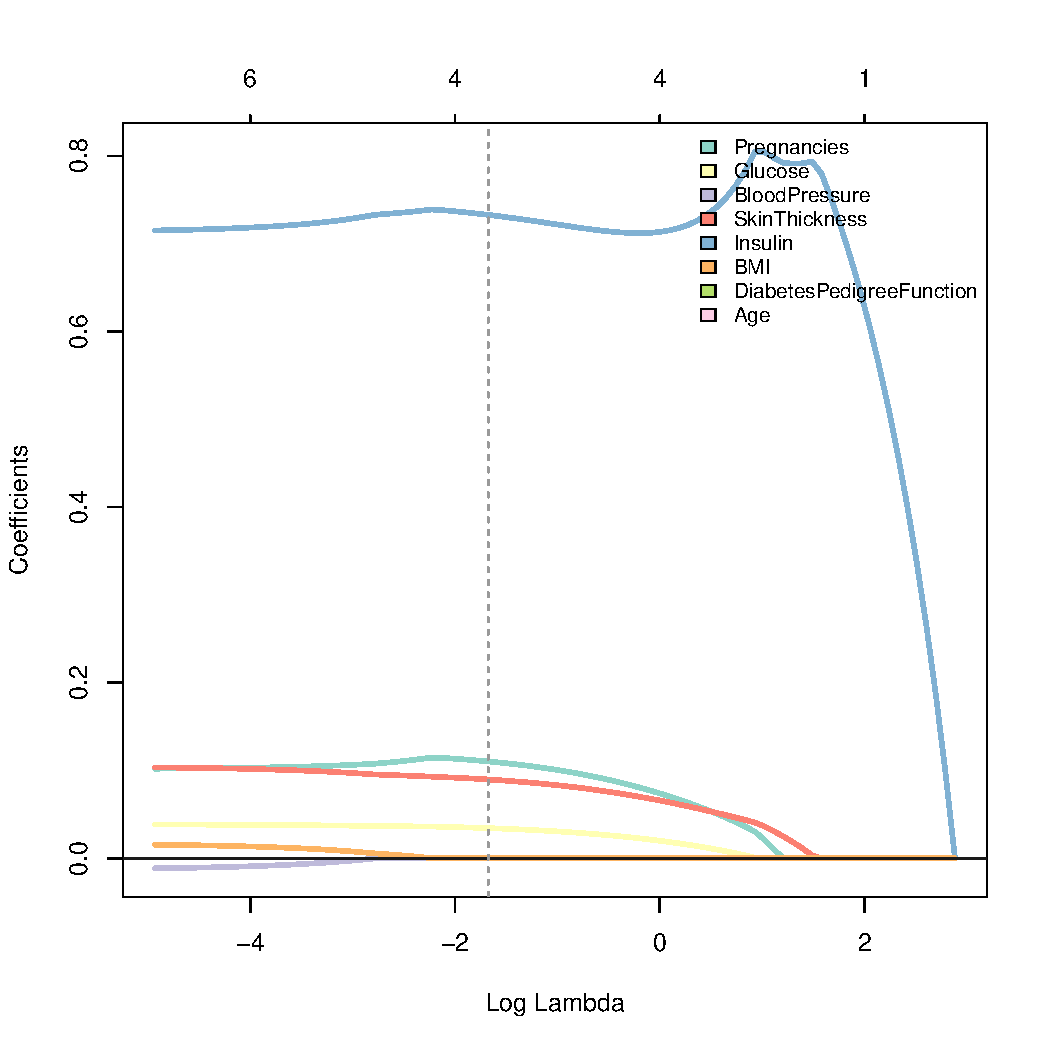
\includegraphics[width=0.85\columnwidth]{plots/diabetes_adalasso.pdf}
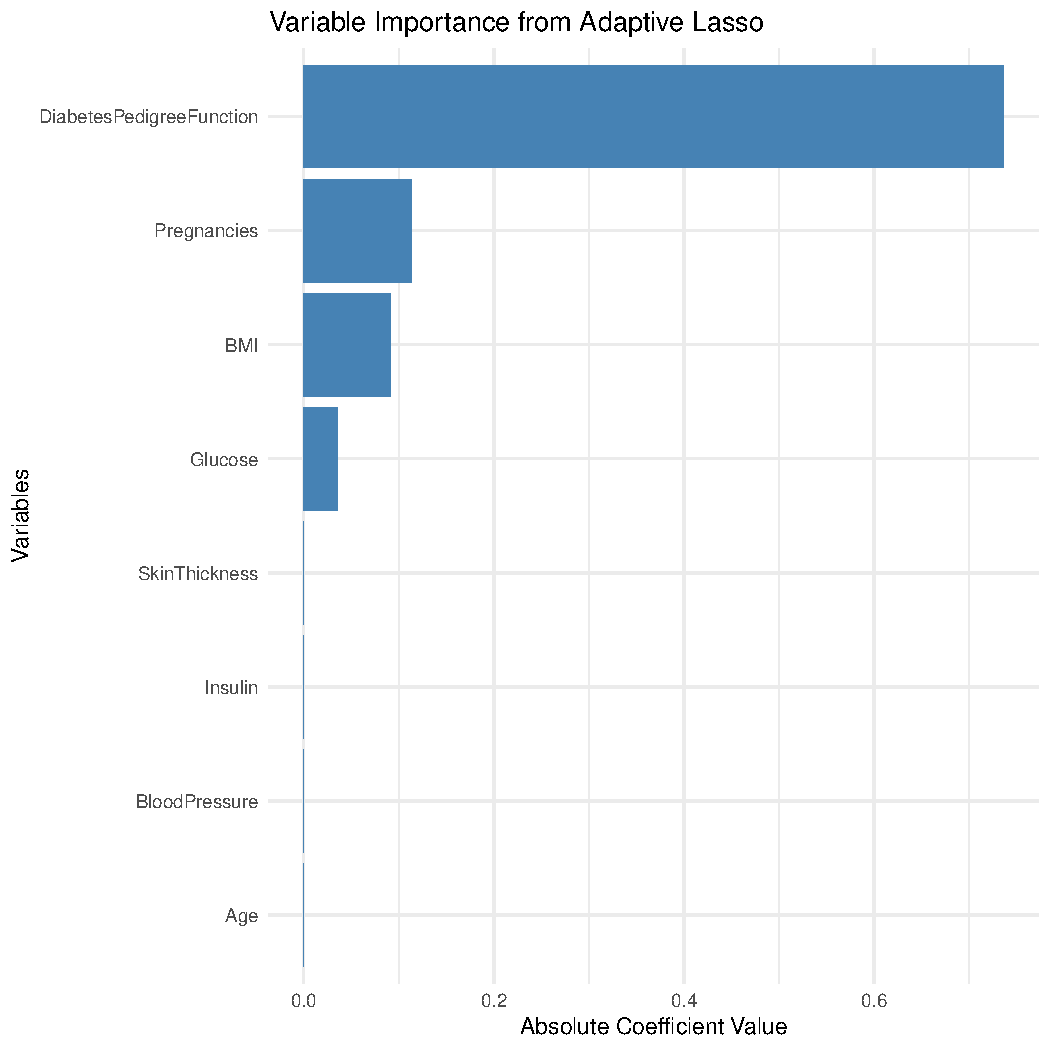
\includegraphics[width=0.7\columnwidth]{plots/variable_importance_adalasso.pdf}
\end{column}
\end{columns}

\end{frame}

\begin{frame}{Results}
    \begin{table}
\sisetup{round-mode=places}
\resizebox{\textwidth}{!}{
\begin{tabular}{lS[round-precision=4]S[round-precision=4]S[round-precision=4]S[round-precision=4]}
	Model & {Train score} & {Test score} & {\(\lambda\)} \\
	\midrule
	Lasso & 0.7714844 & 0.7695312 & 0.005678404 \\
	Ridge & 0.7695312 & 0.765625 & 0.02346324  \\
    ElasticNet & 0.7734375 & 0.7695312 & 0.008591009  \\
    AdaLasso & 0.7714844 & 0.7695312 & 0.005678404 \\
	\bottomrule
\end{tabular}}
\end{table}
\end{frame}